\documentclass{scrartcl}
\usepackage{enumitem}
\RequirePackage[utf8]{inputenc}
\RequirePackage[ngerman]{babel}
\RequirePackage[T1]{fontenc}
\RequirePackage{lmodern}
\usepackage{graphicx}
\usepackage{amsmath}


\usepackage{listings}
\usepackage{subfig}
\usepackage{tikz}
\usetikzlibrary{positioning}

\usepackage{typearea}
\areaset[5mm]{135mm}{237mm}

\begin{document}

\begin{figure}
\centering
\begin{tikzpicture}
\coordinate (a) at (-5,0) node[below=0.1cm of a]{-1000};
\coordinate (b) at (-1,0) node[below=0.1cm of b]{-1};
\coordinate (c) at (0,0) node[below=0.1cm of c]{0};
\coordinate (d) at (1,0) node[below=0.1cm of d]{1};
\coordinate (e) at (5,0) node[below=0.1cm of e]{1000};
\coordinate (f) at (-6,0) node[below=0.1cm of f, xshift=3.0cm]{[...]};
\coordinate (g) at (6,0) node[below=0.1cm of g, xshift=-3.0cm]{[...]};
\fill (a) circle (2.5pt);
\fill (b) circle (2.5pt);
\fill (d) circle (2.5pt);
\fill (e) circle (2.5pt);
\draw (f)--(a)--(b)--(c)--(d)--(e)--(g);
% links 1.
\coordinate (aa) at (-5,0.8);
\draw (a) -- (aa);
\draw (-5,0.8) -- (-5.2,0.8);
\draw (-5.2,0.9) -- (-5.4,0.8) -- (-5.2,0.7) -- cycle;
% links 2.
\coordinate (bb) at (-1,0.8);
\draw (b) -- (bb);
\draw (-1,0.8) -- (-1.7,0.8);
\draw (-1.7,0.9) -- (-1.9,0.8) -- (-1.7,0.7) -- cycle;
% mitte
\draw (0,2) -- (0,1.5) -- (0.4,1.75) -- cycle;
\coordinate (cc) at (0,2);
\draw (c) -- (cc);
% rechts 2.
\coordinate (dd) at (1,0.8);
\draw (d) -- (dd);
\draw (1,0.8) -- (1.7,0.8);
\draw (1.7,0.9) -- (1.9,0.8) -- (1.7,0.7) -- cycle;
% rechts 1.
\coordinate (ee) at (5,0.8);
\draw (e) -- (ee);
\draw (5,0.8) -- (5.2,0.8);
\draw (5.2,0.9) -- (5.4,0.8) -- (5.2,0.7) -- cycle;
\end{tikzpicture}
%\caption{einfaches Gegenspiel}
\label{fig:BSP}
\end{figure}

\begin{figure}
\centering
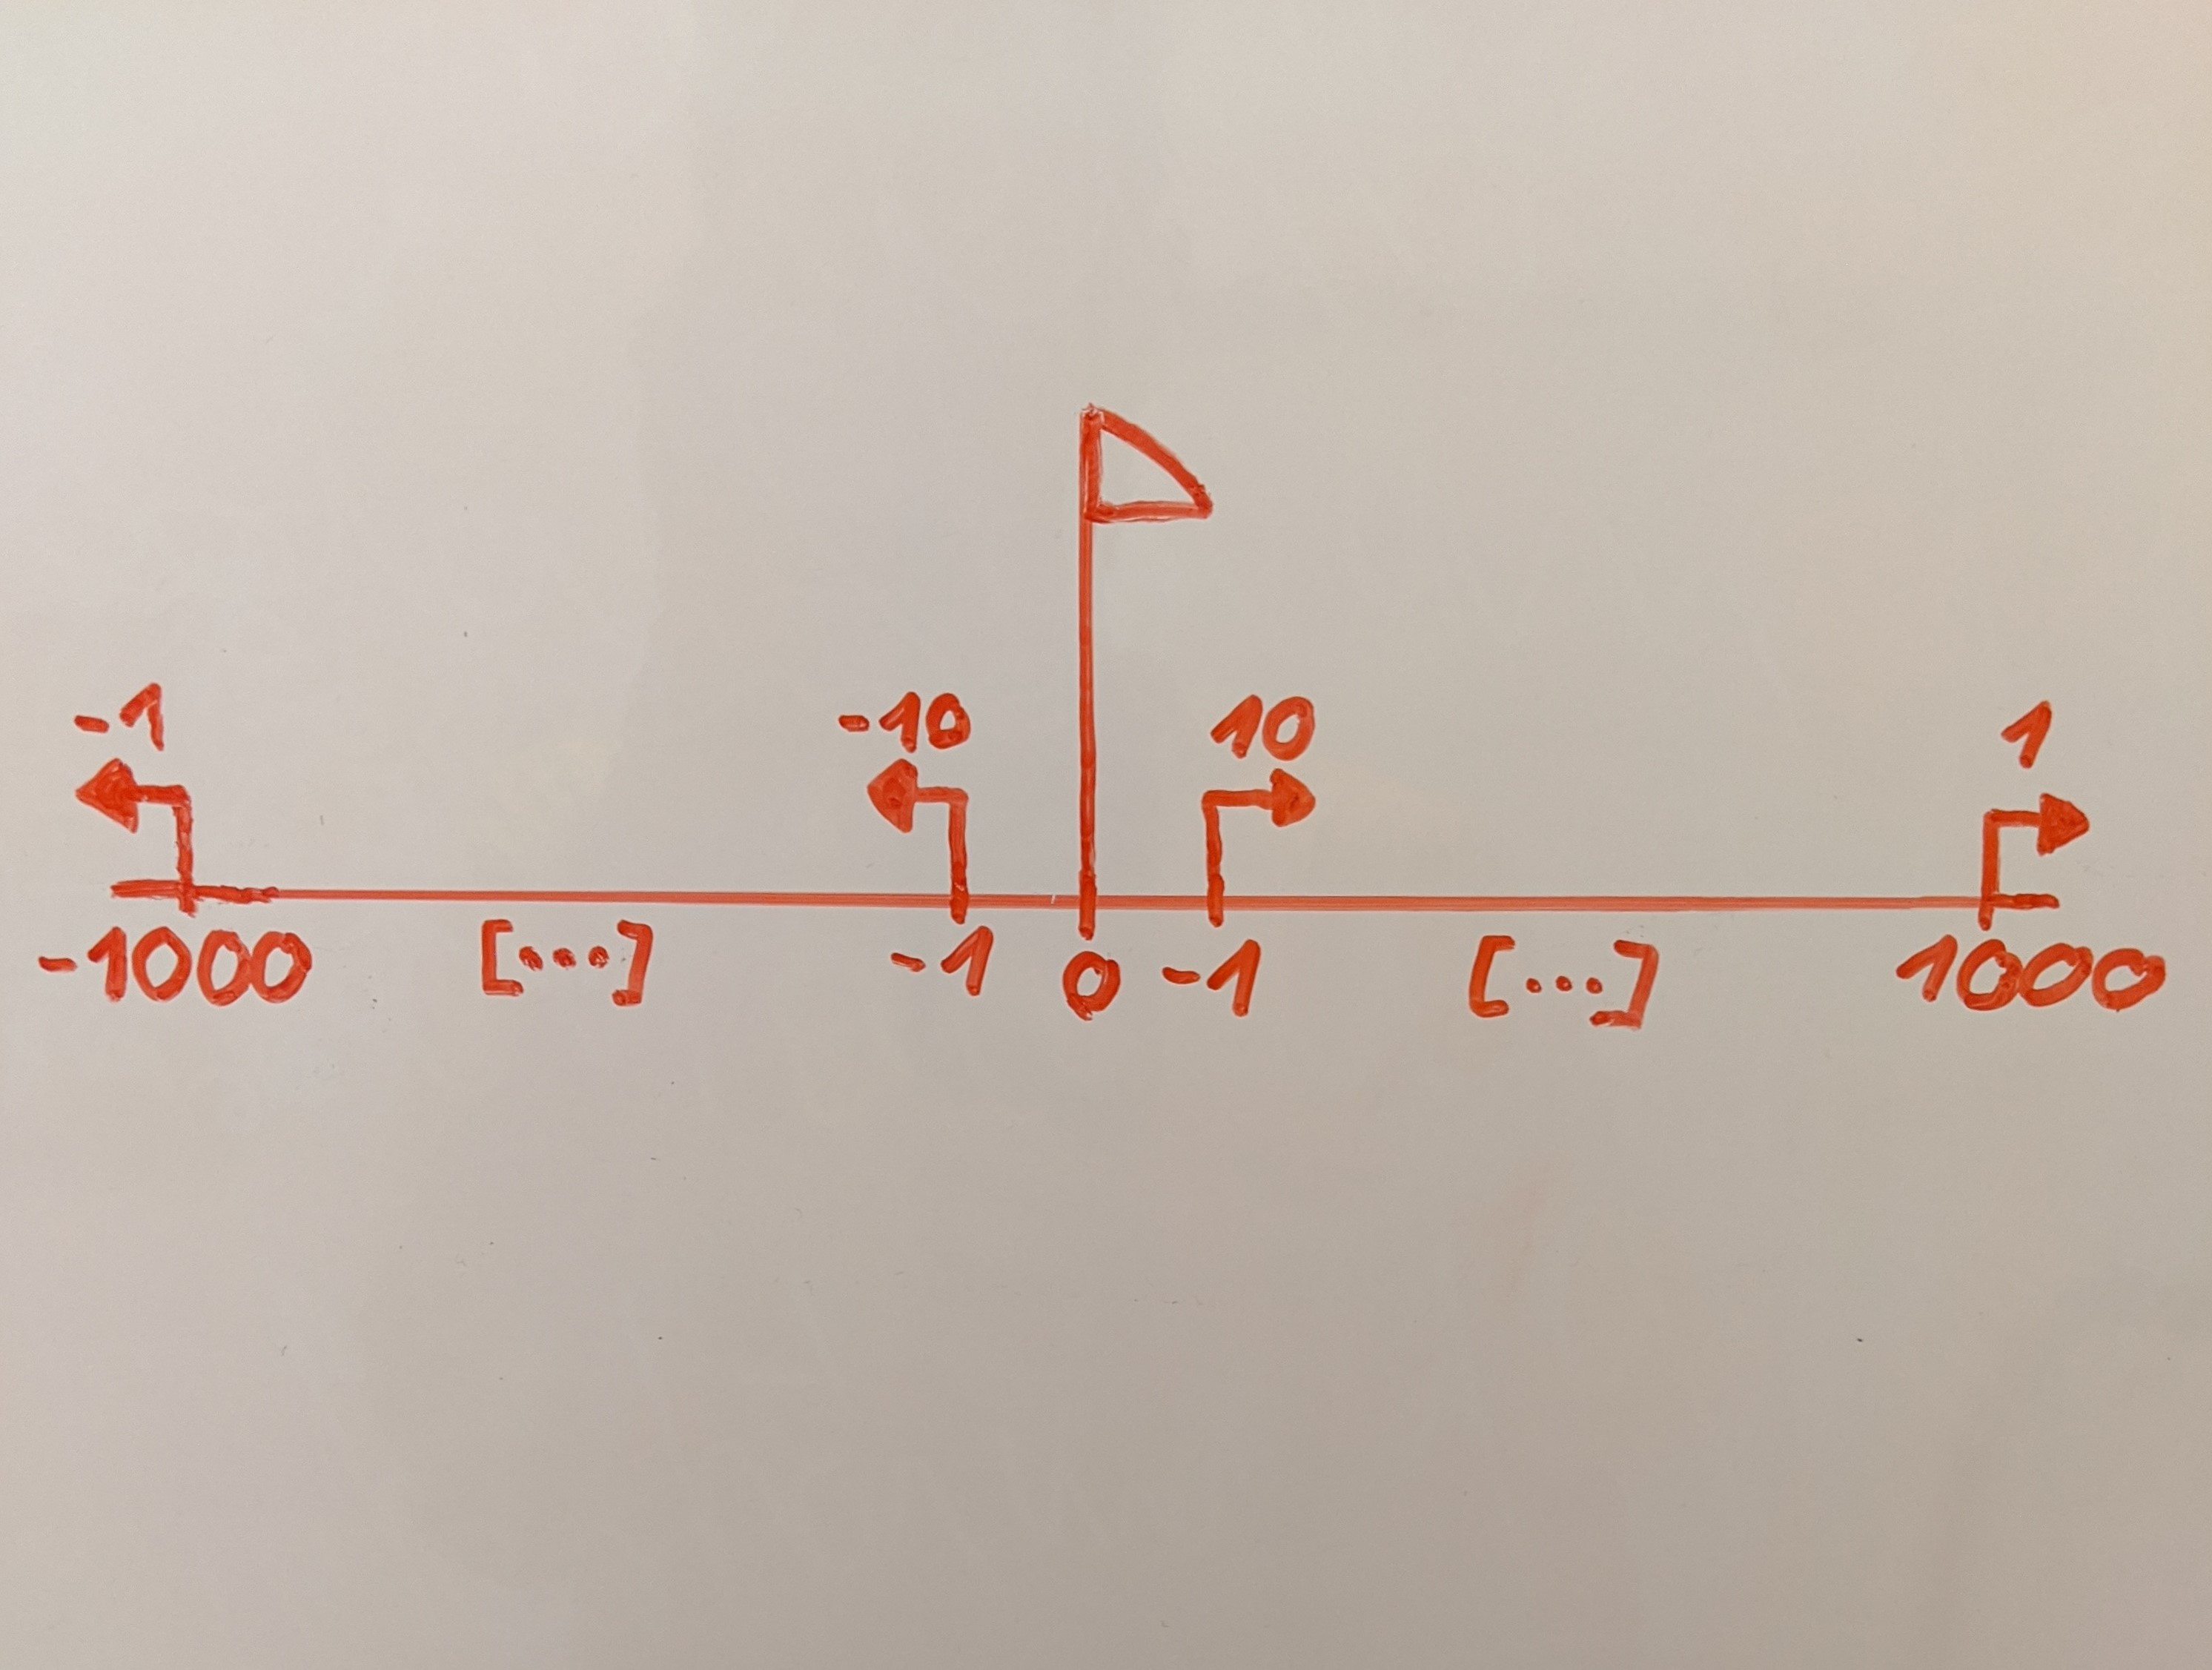
\includegraphics[scale=0.09]{../Grafiken/Whiteboard/GegenBsp1Dim.jpg}
%\caption{einfaches Gegenspiel}
\label{fig:GegenBsp1Dim}
\end{figure}

\end{document}

%\draw[very thick] (-6,0) -- (6,0);
%\draw (0,0) -- (0,2); 